\section{Shared caching layer}\label{section:applied-methods:shared-caching-layer}

The previous section explained how the communication strategy within the micro-frontend architecture works behind the scenes. Apollo Client's caching mechanism should be used to boost the performance of the micro-frontend architecture and handle the problems of over-fetching and over-requesting. This section goes into more detail, how the shared caching layer is implemented and integrated into the architecture. The structure of the shared caching layer is shown in Figure \ref{fig:applied-methods:structure-shared-caching-layer}. Each micro-frontend has a separate instance of the Apollo Client, but they should all use the same instance of the \texttt{InMemoryCache}. Therefore, each application can provide its own configuration for the Apollo Client, however all micro-frontend use the same instance of the \texttt{InMemoryCache}. The \texttt{InMemoryCache} stores the results of GraphQL queries. When a micro-frontend needs to retrieve a query that is already cached, it can reuse the data that is already cached instead of retrieving it again from the GraphQL \ac{API} again. This caching strategy reduces the number of network requests and thus the amount of data that has to be transferred over the network.

\ifshowImages
  \begin{figure}[H]
  \centering
  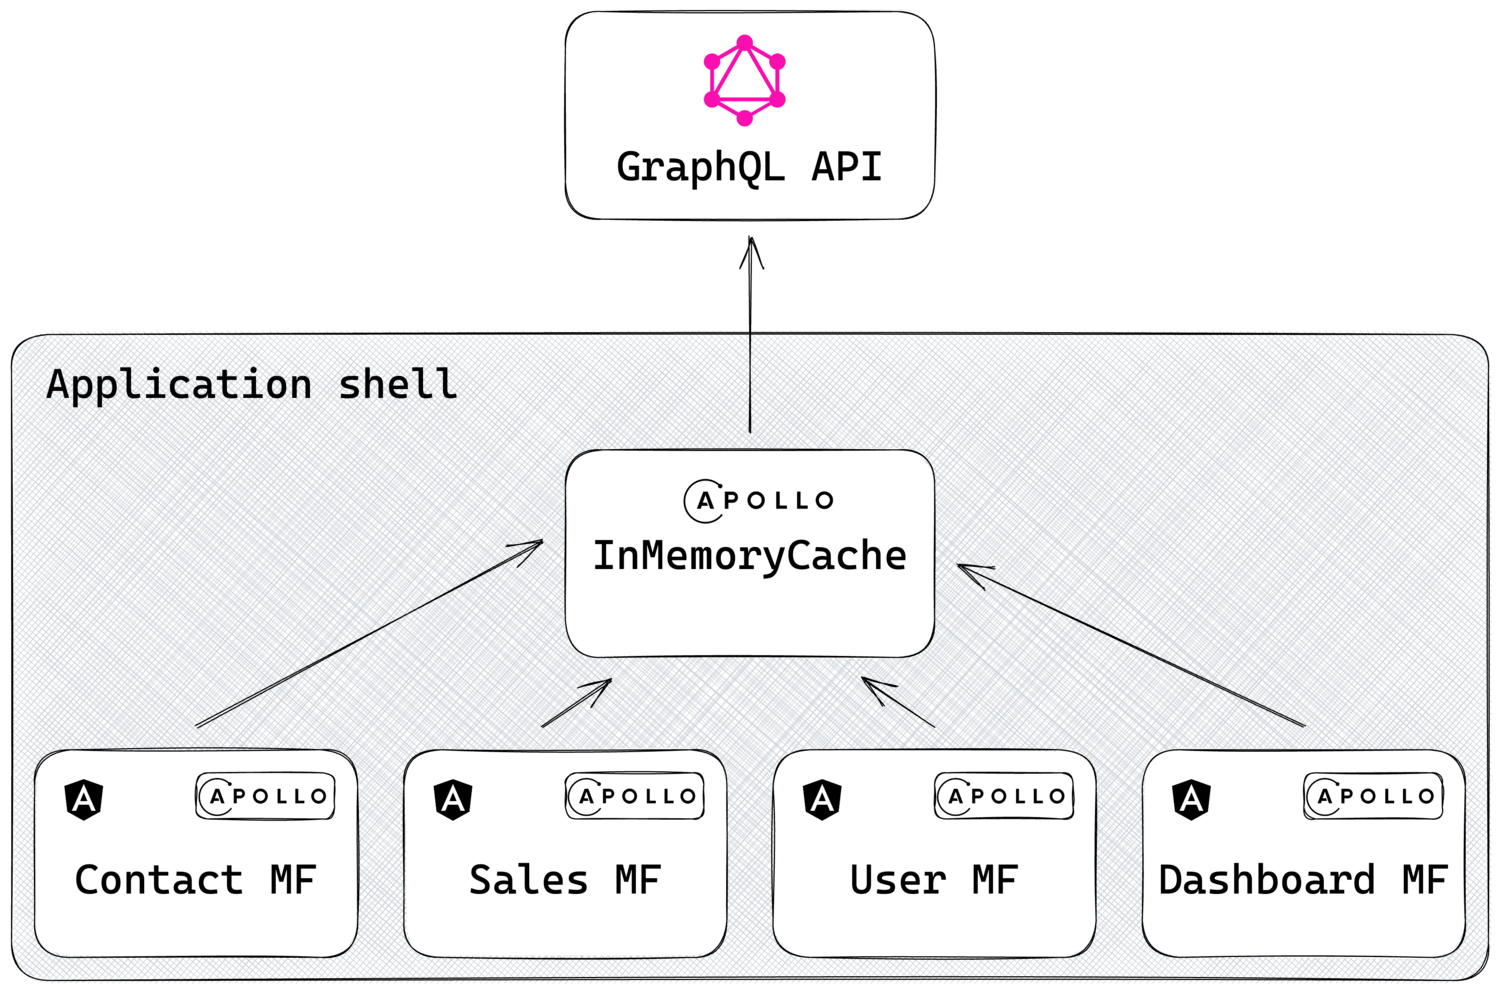
\includegraphics[width=0.7\linewidth]{images/applied-methods/shared-caching-layer/shared-caching-layer.png}
  \caption{The structure of the shared caching layer.}\label{fig:applied-methods:structure-shared-caching-layer}
  \end{figure}
\fi

\noindent The application shell must provide the instance of the GraphQL \texttt{InMemoryCache} to make sure that all micro-frontends have the same instance. Listing \ref{code:applied-methods:creating-the-apollo-client} shows how the Apollo Client is created for an Angular application with default settings. The \texttt{cache} property is important, as it needs an instance of Apollo's \texttt{InMemoryCache}. This allows for the architecture to create a single cache instance elsewhere and pass it to the Apollo Client. 

\ifshowListings
\begin{listing}[H]
\begin{minted}{typescript}
@NgModule({
  imports: [ApolloModule],
  providers: [{
    provide: APOLLO_OPTIONS,
    useFactory: (httpLink: HttpLink) => ({
      cache: new InMemoryCache(),
      link: httpLink.create({ uri: 'http://localhost:3000' }),
    }),
    deps: [HttpLink],
  }]
})
class AppModule {}
\end{minted}
\caption{Create a new instance of the Apollo Client.}\label{code:applied-methods:creating-the-apollo-client}
\end{listing}
\fi

\noindent The concept behind the shared caching layer is to instantiate the cache instance inside the application shell and provide it to the micro-frontends. The instance of the \texttt{InMemoryCache} should be injectable through an injection token, just like the injection token from Section \ref{section:applied-methods:communication-shell-remote}, which specifies whether the application runs in standalone mode. The injection token can be provided by the application shell and injected and used by the micro-frontends. Moreover, the application itself can provide the instance of the cache when it runs in standalone mode. The \texttt{GRAPHQL\_CLIENT\_CACHE} token can be used to provide an instance of Apollo's \texttt{InMemoryCache} to the micro-frontends, as shown in Listing \ref{code:applied-methods:graphql-client-cache-provider}.

\ifshowListings
\begin{listing}[H]
\begin{minted}{typescript}
@NgModule({
  providers: [
    { provide: GRAPHQL_CLIENT_CACHE, useValue: new InMemoryCache() }
  ]
})
class HostCoreModule {}
\end{minted}
\caption{Provide the instance of the \texttt{InMemoryCache} to \ac{DI}.}\label{code:applied-methods:graphql-client-cache-provider}
\end{listing}
\fi

\subsection{GraphQL Client creation}{subsection:applied-methods:shared-caching-layer:graphql-client-creation}

\noindent The prototype provides abstractions to create the necessary configuration for using the Apollo Client more easily and identically for all micro-frontends. Listing \ref{code:applied-methods:graphql-client-creation} shows the usage of the abstraction to create a new instance of Apollo Client for a micro-frontend. The module \texttt{GraphQLClientOptionsModule} hides the complexity of creating and providing a Apollo Client instance, as shown in Listing \ref{code:applied-methods:creating-the-apollo-client-with-a-shared-cache}. The moduls has a required parameter that specifies a unique name. This name is used to identify and track active Apollo Clients inside the architecture. The \texttt{GraphQLClientOptionsModule} should be used in every module that needs GraphQL functionality and is exposed through Module Federation. When the micro-frontend is then integrated within the application shell, it has its own instance of the Apollo Client. This facilitates independent development of micro-frontends, as the Apollo Client configuration remain the same whether it is running in standalone mode or consumed by the application shell. For example, a problem could arise if the application shell provides the instance of the Apollo Client and the contact micro-frontend injects that instance with \ac{DI}. The contact development team might configure the Apollo Client differently within the contact application, and the functionality might not work as expected within the application shell because the configuration might be different.

\ifshowListings
\begin{listing}[H]
  \begin{minted}{typescript}
@NgModule({
  imports: [ GraphQLClientOptionsModule.withConfig('contact-remote') ]
})
class ContactRemoteCoreModule {}
  \end{minted}
  \caption{Create the Apollo Client instance for the micro-frontend.}\label{code:applied-methods:graphql-client-creation}
  \end{listing}
\fi

\ifshowListings
\begin{listing}[H]
\begin{minted}{typescript}
@NgModule({
  imports: [ApolloModule],
  providers: [{
    provide: APOLLO_OPTIONS,
    useFactory(httpLink: HttpLink, cache: InMemoryCache) {
      const link = httpLink.create({uri: 'http://localhost:3000'});
      return { cache, link };
    },
    deps: [HttpLink, GRAPHQL_CLIENT_CACHE],
  }]
})
class ContactRemoteModule {}
  \end{minted}
\caption{Access the shared \texttt{InMemoryCache} instance from \ac{DI}.}\label{code:applied-methods:creating-the-apollo-client-with-a-shared-cache}
\end{listing}
\fi

\noindent The \texttt{GraphQLClientOptionsModule} uses the storage service to get the required configuration for the Apollo Client. For example, \ac{URL} of GraphQL \ac{API} is taken from the storage service. By default, it tries to inject the \texttt{GRAPHQL\_CLIENT\_CACHE}, and use it as the cache instance for the Apollo Client. If it cannot be injected, a separate cache instance is created for the client. An addtional injection token \texttt{GRAPHQL\_CLIENT\_OPTIONS\_CONFIG} can be used to specify additional options for creating a new Apollo Client instance. The injection token's usage and default options are shown inside Listing \ref{code:applied-methods:graphql-client-extra-configuration-options}. The injection token must be provided inside the same module where the \texttt{GraphQLClientOptionsModule} was defined.

\ifshowListings
\begin{listing}[H]
\begin{minted}{typescript}
@NgModule({
  providers: [{
    provide: GRAPHQL_CLIENT_OPTIONS_CONFIG,
    useValue: {
      shareCache: true,
      persistCache: false,
      useTypePolicies: true,
      typePolicies: CONTACT_TYPE_POLICIES,
    },
  }]
})
class ContactRemoteCoreModule {}
\end{minted}
\caption{Provide additional options for creating the Apollo Client instance.}\label{code:applied-methods:graphql-client-extra-configuration-options}
\end{listing}
\fi

\noindent The options include \texttt{shareCache}, \texttt{persistCache}, \texttt{useTypePolicies} and \texttt{typePolicies}. The \texttt{shareCache} setting is used to specify whether the Apollo Client should use the \texttt{InMemoryCache} instance provided by \texttt{GRAPHQL\_CLIENT\_CACHE} or if it should create a new instance, specifically for this remote module. The \texttt{persistCache} option is set to \texttt{false} by default. It stores the contents of the \texttt{InMemoryCache} inside the \texttt{localStorage}. This feature provided by the Apollo Client allows faster initial page renders, because the data from the \texttt{localStorage} is transferred back to the cache when the application is loaded. The options \texttt{useTypePolicies} and \texttt{typePolicies} are used together and must be specified together. The property \texttt{useTypePolicies} specifies whether the type policies from the option \texttt{typePolicies} should be used or not. Type policies allow Apollo Client to customize the read and write operations of every field inside the cache. They are explained in more detail in Section \ref{subsubsection:background:graphql:apollo-server-client:type-policies}. As explained earlier, each micro-frontend has its own Apollo client instance with a shared cache instance, so the type policies cannot be registered directly when the \texttt{InMemoryCache} is created. The option \texttt{typePolicies} has the same type as the \texttt{typePolicies} parameter of the \texttt{InMemoryCache} constructor. Specifying the option when providing the \texttt{GRAPHQL\_CLIENT\_OPTIONS\_CONFIG} allows the micro-frontend to specify additional type policies for the cache. Part of the code to create the shared cache and append type-policies within the \texttt{GraphQLClientOptionsModule} is shown in Listing \ref{code:applied-methods:adding-extra-type-policies}. First, the instance of the cache should be injected. If the cache cannot be injected, it means that the Apollo Client has to create a new instance of the \texttt{InMemoryCache}. The \texttt{typePolicies} are added to the cache instnace if both options \texttt{typePolicies} and \texttt{useTypePolicies} are truthy values.

\ifshowListings
\begin{listing}[H]
\begin{minted}{typescript}
const cache = inject(GRAPHQL_CLIENT_CACHE, { optional: true });
const { shareCache, useTypePolicies, typePolicies } = graphQLClientOptions;

const cacheInstance = shareCache ? cache : new InMemoryCache();

if (typePolicies && useTypePolicies)
  clientCache.policies.addTypePolicies(typePolicies);
\end{minted}
\caption{Insert additional type policies into the cache instance.}\label{code:applied-methods:adding-extra-type-policies}
\end{listing}
\fi
